\section{Software}

\subsection{Methodology}

In the past, software projects followed a strict-plan driven approach, such as the Waterfall method, however more recently, Agile practices have become widely accepted, allowing the developer more freedom. This features an iterative development approach, with short \say{iterations} or \say{sprints} defined in which the developer should complete a block of work, typically a \say{story} or \say{feature} given the Agile methodology chosen.

The Agile Methodology has a manifesto \cite{Manifesto}, which perfectly encompasses all the values it strives to achieve:
\begin{itemize}
  \item \textbf{Individuals and interactions} over processes and tools
  \item \textbf{Working software} over comprehensive documentation
  \item \textbf{Customer collaboration} over contract negotiation
  \item \textbf{Responding to change} over following a plan
\end{itemize}

\begin{quotation}
  \textit{That is, while there is value in the items on the right, we value the items on the left more.}
\end{quotation}

Scrum is one of the most popular interpretations of an Agile Methodology, due to it's simplicity \cite{scrum}. Scrum is \textit{not} an agile methodology, however is a framework, to which agile practices such as Pair Programming and \acrfull{TDD} can be aligned.

Given it's flexible and light-weight nature, an adapted Scrum methodology has been undertaken for this project.


\subsubsection{Tools to manage methodology}

This project has been chiefly supported by the tool \url{taiga.io} - a beta web app \cite{Taiga.io}, which aims to promote the use of Scrum and Kanban \cite{kanban}.

\subsubsection{Burn down chart}
\subsubsection{User stories}

User Stories are a bid to shift away from talking in technical-jargon, and to shift towards talking in plain english about project requirements. When working with a customer, this is obviously useful, as occasionally they can be non-technical, so this helps promote an open-dialogue between customer and developer, and a clear understanding of the customer's needs.

User Stories typically follow a template for consistency, usually something similar to:

\begin{quotation}
  \textit{As a $<$type of user$>$, I want $<$some goal$>$ so that $<$some reason$>$.} \cite{user_story}
\end{quotation}

Table \ref{table:User Stories} outlines the User Stories used during this project, along with when they were working upon (during which Sprint) and which/how many tasks were associated with it.

\begin{center}
  \small
  \begin{longtable}{| p{2cm} | p{4cm} | p{2cm}  | p{2cm} | p{3cm} |}
    \hline
      \textbf{Reference} & \textbf{User Story} & \textbf{Milestone} & \textbf{Associated Tasks} & \textbf{Comments} \\ \hline \endhead
      1 & Clinicians can upload a set of images (MATLAB Command Window) so they can control what images are input into the Congealing Algorithm & Sprint 0 & 13, 14 & \\ \hline
      2 & Developer will implement membership of a pixel so that Fuzzy Entropy can be calculated & Sprint 1 & 19, 20, 21 & \\ \hline
      3 & Clinicians can align scans using Non-Probabilistic Entropy so it can be used in the Congealing Algorithm & Sprint 2 \& 3 & 22, 24, 25, 32, 52 & Due to complexity of the implementation, this was spread over 2 sprints \\ \hline
      4 & Clinicians can select an alignment metric (MATLAB Command Window) so they can select which to align the images using & Sprint 4 & 41, 42, 43 & \\ \hline
      5 & Developer will make standard GUI with no functionality so that this can be demoed as a proof of concept & Sprint 4 & 34, 35, 36, 37, 38, 39, 40 & \\ \hline
      6 & Clinician can choose number of iterations (MATLAB Command Window) so they can run as many as they want to & Sprint 4 & 45, 46, 47 & \\ \hline
      7 & Developer will implement Basic mammogram upload so that they can be aligned & Sprint 4 & 49, 50, 51, 55 & \\ \hline
      8 & Clinicians can align scans using standard Entropy so it can be used in the Congealing Algorithm & Sprint 5 & 56 & \\ \hline
      9 & Clinicians can upload a set of images - GUI & Sprint 5 & 61, 62, 63 & \\ \hline
      10 & Developer will optimise membership function so as to improve performance & Sprint 5 & 58, 59 & Promoted from an Issue \\ \hline
      11 & Developer will optimise Non-Probabilistic Function so as to improve performance & Sprint 5 & 60 & Promoted from an Issue \\ \hline
      12 & Clinicians can clear an input image so that they can reselect an input image & Sprint 5 & 65 & \\ \hline
      13 & Clinicians can align scans using Hybrid Entropy so it can be used in the Congealing Algorithm  & Sprint 6 & 74, 75, 76 & \\ \hline
      14 & Clinicians can select an alignment metric from a drop-down menu so it is easy to choose which alignment metric to use & Sprint 6 & 68, 69 & \\ \hline
      15 & Clinicians can select the number of iterations to be run using an alignment metric (GUI) so it is easy to select how many iterations to run & Sprint 6 & 70, 71, 72, 73 & \\ \hline
      16 & Clinicians can see meta data about the input image so they can see if the uploaded image is the correct one & Sprint 6 & 85, 86, 87 & \\ \hline
      17 & Clinicians can see each iteration mean image so they can compare the improvement over each iteration & Sprint 6 & 81, 82, 83, 84 & \\ \hline
      18 & Clinicians can see adjusted input images on final iteration so they can see how the input images have changed by the final iteration & Sprint 6 & 88, 89, 90 & \\ \hline
      19 & Developer wants to know why Scans are rotated 90 to left as this is aesthetically displeasing & Sprint 7 & 100, 101, 102 & Promoted from an Issue \\ \hline
      20 & Developer will research and implement removal of Medical Markers as this causes alignment issues & Sprint 7 & 96, 97, 98, 99 & \\ \hline
      21 & Clinicians can discard (clear) an alignment so they can start a new alignment & Sprint 8 & 110, 111, 112, 113, 114 & \\ \hline
      22 & Clinicians can click on average image to view it bigger so they can see the detail easier & Sprint 8 & 105, 106 & \\ \hline
      23 & Clinicians can save the final mean image with a sensible name so they can easily find it again & Sprint 8 & 107, 108, 109 & \\ \hline
      24 & Clinicians can see the iteration details so they can understand more about the improvement & Sprint 8 & 115, 116, 117, 118, 119, 120, 121 & \\ \hline
      25 & Clinicians can see congealing is running so they know it's in progress & Sprint 8 & 123, 124 & \\ \hline
  \caption{User stories defined during the project}
  \label{table:User Stories}
\end{longtable}
\end{center}

\subsubsection{Sprint Review \& Retrospective}

Sprint Reviews are held at the end of each Sprint, to assess what work was done during the week, and does the end product match the Sprint Goal set out at the start of the week. In this project, Sprint Goals and Sprint Reviews took shape in the form of an informal online blog. Weekly posts would outline what had been completed that week, and what was to be completed during the following week. Whilst less structured than the conventional approach to Reviews, it works well within a single-person project, and was a good reflection of what had been accomplished.

In Agile Methodologies, Retrospectives are typically at the end of each Sprint, so the team can assess:
\begin{itemize}
  \item What works well
  \item What doesn't work well
  \item What should they start doing
\end{itemize}

\subsubsection{Daily Standup}

Daily standups are a vital part of Scrum`s teamwork ethos. Each morning (or during a set allotted time), the time would meet to discuss what was accomplished the day before, what are the plans for the day ahead, and what road-blocks are in their way. This provides the developer (and further the team) a clear picture of what has yet to be done, and allows fellow team-mates to offer expertise to help overcome obstacles. Whilst this project is not being developed by a team, the benefit of daily standups to productivity, organisation and planning still stands, along with the crowd-sourcing element of expertise.

Throughout the project, stand ups have been held with peers, who're also working upon their Major Projects. Whilst not daily, they tended to fall bi-daily, and it gave the developer a chance to hone skills in explaining the project to people not well-versed in the subject. It was also a good breeding ground for new ideas, and an open forum for discussion into the pros and cons of certain approaches.


\subsection{Design}

\begin{itemize}
\item CRC cards
\end{itemize}

\subsection{Implementation}

\subsection{Testing}

Prior to the project beginning, it was outlined that this project should follow a \acrshort{TDD} practice. In \acrshort{TDD}, the Developer first writes a test, which will fail due to the lack of corresponding functionality. They would then go on to implement the functionality desired by the test. Finally, any refactoring of the initial test and/or code would take place.

However due to the nature of the research, it became increasingly more difficult to follow given the research which had to be undertaken alongside development. This led to a change from \acrshort{TDD} to Retrospective Testing, in which I would write all tests, post functional implementation. This is a more traditional approach to testing, and still catches the same errors which might occur during \acrshort{TDD}.

\subsubsection{Unit Tests}

Unit Tests were completed using MATLAB`s Unit Testing Framework \cite{testing}, which covers all the ways in which you can program in MATLAB:

\begin{itemize}
  \item Script-Based Unit Tests
  \item Function-Based Unit Tests
  \item Class-Based Unit Tests
  \end{itemize}

The majority of my work in MATLAB was Function-based, so this was the style followed for unit tests.

\begin{figure}[H]
  \centering
  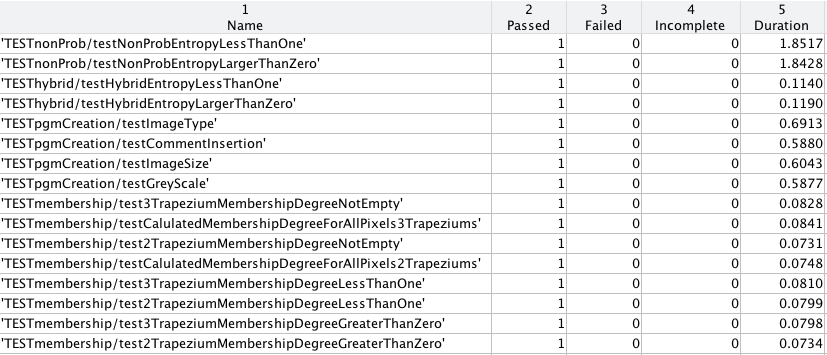
\includegraphics[width=\textwidth]{Chapter2/software-img/test-results.png}
  \caption{Results from MATLAB Unit Tests.}
  \label{fig:unit-test-results}
\end{figure}

As Figure \ref{fig:unit-test-results} demonstrates, all Unit tests passed.

\subsubsection{Acceptance Tests}

Table \ref{table:acceptance} outlines the results from the Acceptance Tests run. The left-most column \say{User Story Reference} aligns with Table \ref{table:User Stories}, so more detail can be found.

\begin{center}
  \small
  \begin{longtable}{| p{3cm} | p{4cm} | p{4cm}  | p{3cm} | p{2cm} |}
    \hline
      \textbf{User Story Reference} & \textbf{Expected Outcome} & \textbf{Actual Outcome} & \textbf{Pass/Fail} \\
      1 & Image is loaded into the system & As expected & Pass \\ \hline
      2 & Membership array is passed out of the membership function and is usable in other functions & As expected & Pass \\ \hline
      3 & Images are aligned using Non-Probabilistic entropy and the output \& entropy outputs are realistic & As expected & Pass \\ \hline
      4 & Images are aligned using the metric the user has selected when running the function & As expected & Pass \\ \hline
      6 & The number of iterations is run as specified by the User, then function stops & As expected & Pass \\ \hline
      8 & Images are aligned using Shannon entropy and the output \& entropy outputs are realistic & As expected & Pass \\ \hline
      9 & Image(s) selected to be loaded into the GUI is displayed & As expected & Pass \\ \hline
      12 & Image box where input image appears goes blank after Clear button is selected & As expected & Pass \\ \hline
      13 & Images are aligned using Hybrid entropy and the output \& entropy outputs are realistic & As expected & Pass \\ \hline
      14 & Images are aligned using the chosen alignment metric & As expected & Pass \\ \hline
      15 & The number of iterations is run as specified by the User, then function stops & As expected & Pass \\ \hline
      16 & When an input image is loaded in, Metadata is displayed in the GUI about the image & As expected & Pass \\ \hline
      17 & After Congealing, the user can press the \say{See all Mean images} button and a new Figure displays the mean image after each iteration & As expected & Pass \\ \hline
      18 & After Congealing, the user can press the \say{See Adjusted Inputs} button and a new Figure displays the adjusted input images after the final iteration  & As expected & Pass \\ \hline
      21 & Image box where output image appears goes blank after Clear button is selected along with all other fields & As expected & Pass \\ \hline
      22 & Image is displayed larger in a new Figure & As expected & Pass \\ \hline
      23 & Save file dialog appears with a sensible name suggested (i.e. final image - alignment-chosen - number of iterations) & As expected & Pass \\ \hline
      24 & When \say{Entropy details} button is selected, a new Figure appears with a graph showing entropy decrease. Final Entropy \& time taken also displays in the main GUI & As expected & Pass \\ \hline
      25 & Egg-timer appears when Congealing Algorithm is running & As expected & Pass \\ \hline
      \caption{Acceptance Test results}
      \label{table:acceptance}
  \end{longtable}
\end{center}
